\documentclass[12pt]{article}  
%%Read the manual for other options. 

\pagestyle{empty} %%Eliminates page numbers
%%\input rmb_macros
%%Collect your favorite macros in a 
%%separate file

%\input amssym.def
%\input amssym
%\input mssymb
%%Defines additional symbols



\usepackage{graphics}
\usepackage{amsmath,amssymb,amsthm, multicol,tikz,pgf,subfig,enumerate}
\usetikzlibrary{arrows.meta}
%\usepackage[pdftex]{graphicx}
\usepackage{epsf}
%%Use to include pictures. 

%\newcommand{\comment}[1]{}
%\newcommand{\sobolev}[2]{W^{#1,#2}}
%\newcommand{\sobolev}[2]{L^#2_#1}
%%Some examples of macros or new commands.

%\addtolength{\oddsidemargin}{-.75in}
%\addtolength{\evensidemargin}{-.75in}
%\addtolength{\textwidth}{1.5in}
%\addtolength{\topmargin}{-1in}
%\addtolength{\textheight}{2.25in}
%%Set margins, defaults are ok. 

\begin{document}
% \begin{center}
% {\bf \Large Public-Key Cryptography}
% \vspace{0.2cm}
% \hrule
% \end{center}


% \newpage
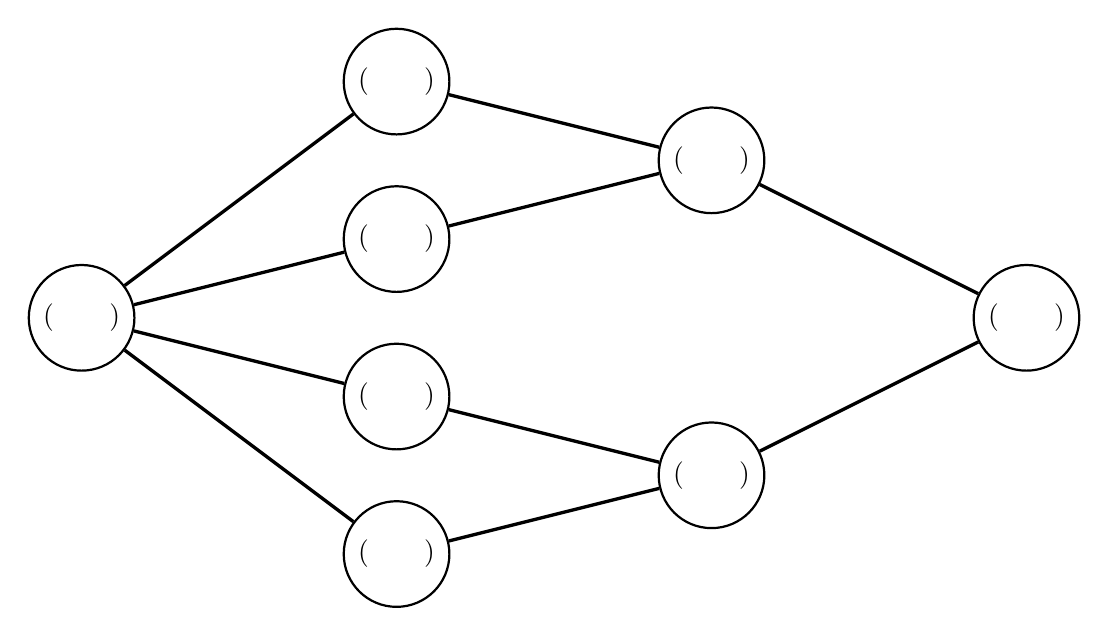
\begin{tikzpicture}
\begin{scope}[every node/.style={circle,thick,draw}]
    \node (v1) at (0,3) {(\qquad)};
    \node (v2) at (4,0) {(\qquad)};
    \node (v3) at (4,2) {(\qquad)};
    \node (v4) at (4,4) {(\qquad)};
    \node (v5) at (4,6) {(\qquad)};
    \node (v6) at (8,1) {(\qquad)};
    \node (v7) at (8,5) {(\qquad)};
    \node (v8) at (12,3) {(\qquad)};
\end{scope}

\begin{scope}[every node/.style={fill=white,circle},
              every edge/.style={draw=black,very thick}]
    \path (v1) edge (v2);
    \path (v1) edge (v3);
    \path (v1) edge (v4);
    \path (v1) edge (v5);
    \path (v2) edge (v6);
    \path (v3) edge (v6);
    \path (v4) edge (v7);
    \path (v5) edge (v7);
    \path (v6) edge (v8);
    \path (v7) edge (v8);
\end{scope}
\end{tikzpicture}

\vspace{2cm}
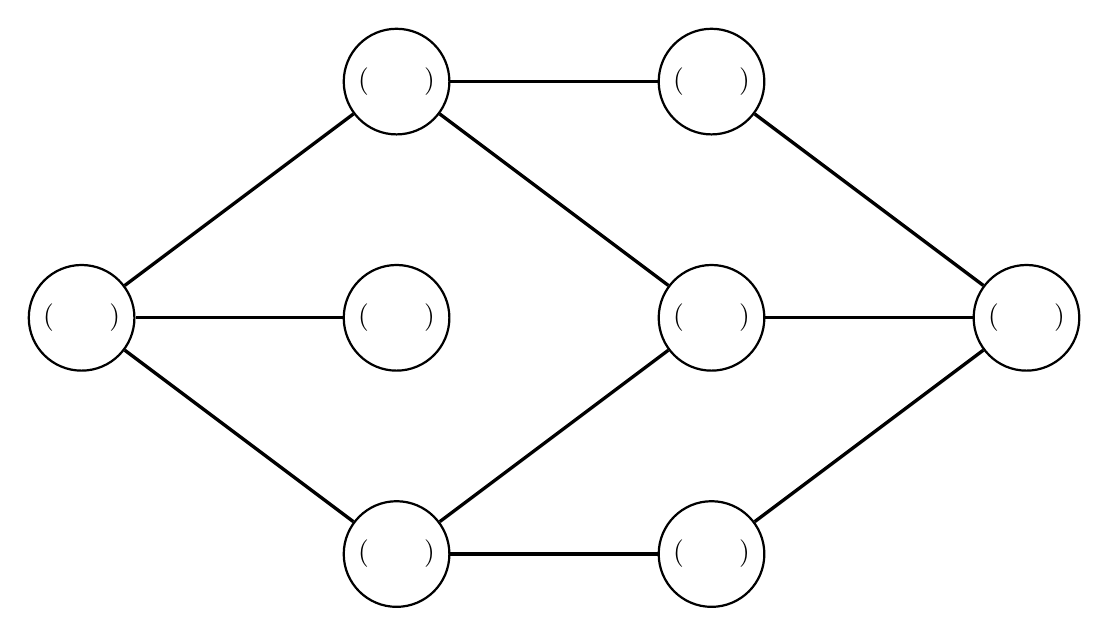
\begin{tikzpicture}
\begin{scope}[every node/.style={circle,thick,draw}]
    \node (v1) at (0,3) {(\qquad)};
    \node (v2) at (4,0) {(\qquad)};
    \node (v3) at (4,3) {(\qquad)};
    \node (v4) at (4,6) {(\qquad)};
    \node (v5) at (8,0) {(\qquad)};
    \node (v6) at (8,3) {(\qquad)};
    \node (v7) at (8,6) {(\qquad)};
    \node (v8) at (12,3) {(\qquad)};
\end{scope}

\begin{scope}[every node/.style={fill=white,circle},
              every edge/.style={draw=black,very thick}]
    \path (v1) edge (v2);
    \path (v1) edge (v3);
    \path (v1) edge (v4);
    \path (v2) edge (v5);
    \path (v2) edge (v6);
    \path (v4) edge (v6);
    \path (v4) edge (v7);
    \path (v5) edge (v8);
    \path (v6) edge (v8);
    \path (v7) edge (v8);
\end{scope}
\end{tikzpicture}


\newpage
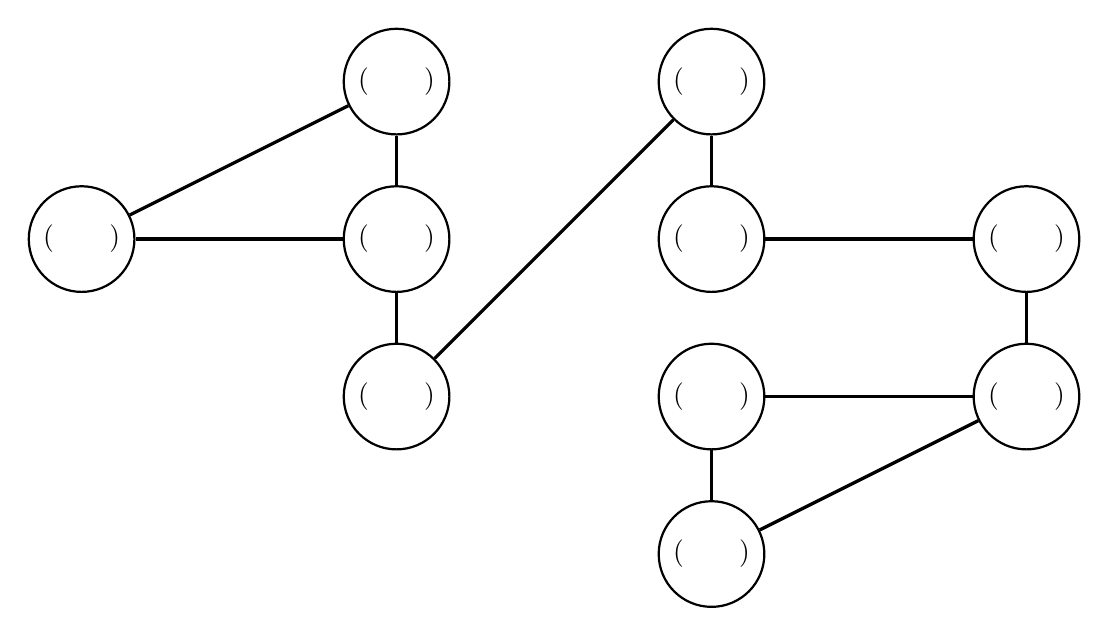
\begin{tikzpicture}
\begin{scope}[every node/.style={circle,thick,draw}]
    \node (v1) at (0,4) {(\qquad)};
    \node (v2) at (4,2) {(\qquad)};
    \node (v3) at (4,4) {(\qquad)};
    \node (v4) at (4,6) {(\qquad)};
    \node (v5) at (8,0) {(\qquad)};
    \node (v6) at (8,2) {(\qquad)};
    \node (v7) at (8,4) {(\qquad)};
    \node (v8) at (8,6) {(\qquad)};
    \node (v9) at (12,2) {(\qquad)};
    \node (v10) at (12,4) {(\qquad)};
\end{scope}

\begin{scope}[every node/.style={fill=white,circle},
              every edge/.style={draw=black,very thick}]
    \path (v1) edge (v3);
    \path (v1) edge (v4);
    \path (v2) edge (v3);
    \path (v3) edge (v4);
    \path (v2) edge (v8);
    \path (v5) edge (v6);
    \path (v5) edge (v9);
    \path (v6) edge (v9);
    \path (v7) edge (v8);
    \path (v7) edge (v10);
    \path (v9) edge (v10);
\end{scope}
\end{tikzpicture}

\vspace{2cm}
\centering
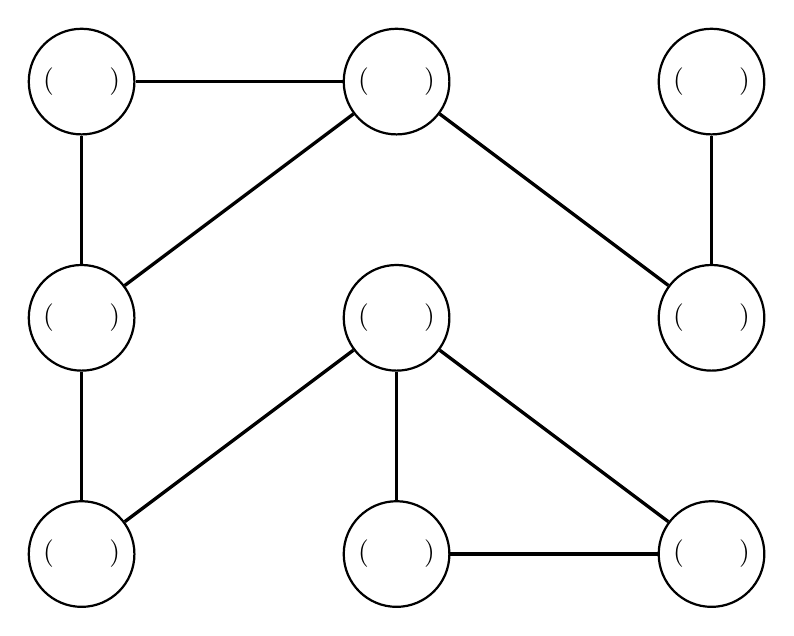
\begin{tikzpicture}
\begin{scope}[every node/.style={circle,thick,draw}]
    \node (v1) at (0,0) {(\qquad)};
    \node (v2) at (0,3) {(\qquad)};
    \node (v3) at (0,6) {(\qquad)};
    \node (v4) at (4,0) {(\qquad)};
    \node (v5) at (4,3) {(\qquad)};
    \node (v6) at (4,6) {(\qquad)};
    \node (v7) at (8,0) {(\qquad)};
    \node (v8) at (8,3) {(\qquad)};
    \node (v9) at (8,6) {(\qquad)};
\end{scope}
\begin{scope}[every node/.style={fill=white,circle},
              every edge/.style={draw=black,very thick}]
    \path (v1) edge (v2);
    \path (v1) edge (v5);
    \path (v2) edge (v3);
    \path (v2) edge (v6);
    \path (v3) edge (v6);
    \path (v4) edge (v5);
    \path (v4) edge (v7);
    \path (v5) edge (v7);
    \path (v6) edge (v8);
    \path (v8) edge (v9);
\end{scope}
\end{tikzpicture}

\newpage

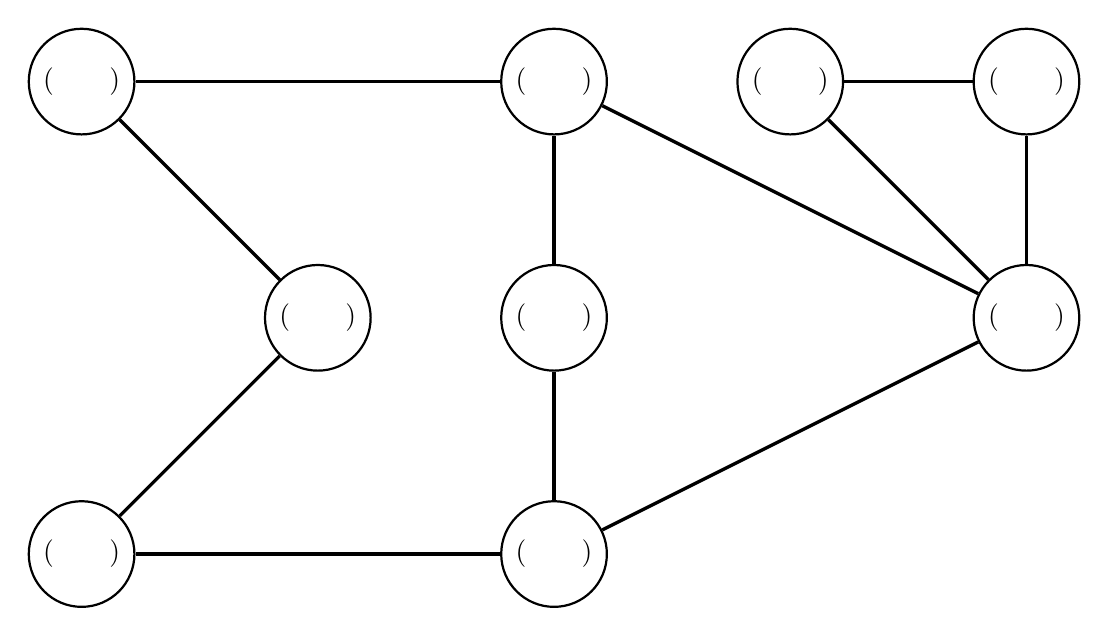
\begin{tikzpicture}
\begin{scope}[every node/.style={circle,thick,draw}]
    \node (v1) at (0,0) {(\qquad)};
    \node (v2) at (0,6) {(\qquad)};
    \node (v3) at (3,3) {(\qquad)};
    \node (v4) at (6,0) {(\qquad)};
    \node (v5) at (6,3) {(\qquad)};
    \node (v6) at (6,6) {(\qquad)};
    \node (v7) at (9,6) {(\qquad)};
    \node (v8) at (12,3) {(\qquad)};
    \node (v9) at (12,6) {(\qquad)};
\end{scope}
\begin{scope}[every node/.style={fill=white,circle},
              every edge/.style={draw=black,very thick}]
    \path (v1) edge (v3);
    \path (v1) edge (v4);
    \path (v2) edge (v3);
    \path (v2) edge (v6);
    \path (v4) edge (v5);
    \path (v4) edge (v8);
    \path (v5) edge (v6);
    \path (v6) edge (v8);
    \path (v7) edge (v8);
    \path (v7) edge (v9);
    \path (v8) edge (v9);
\end{scope}
\end{tikzpicture}


\vspace{2cm}

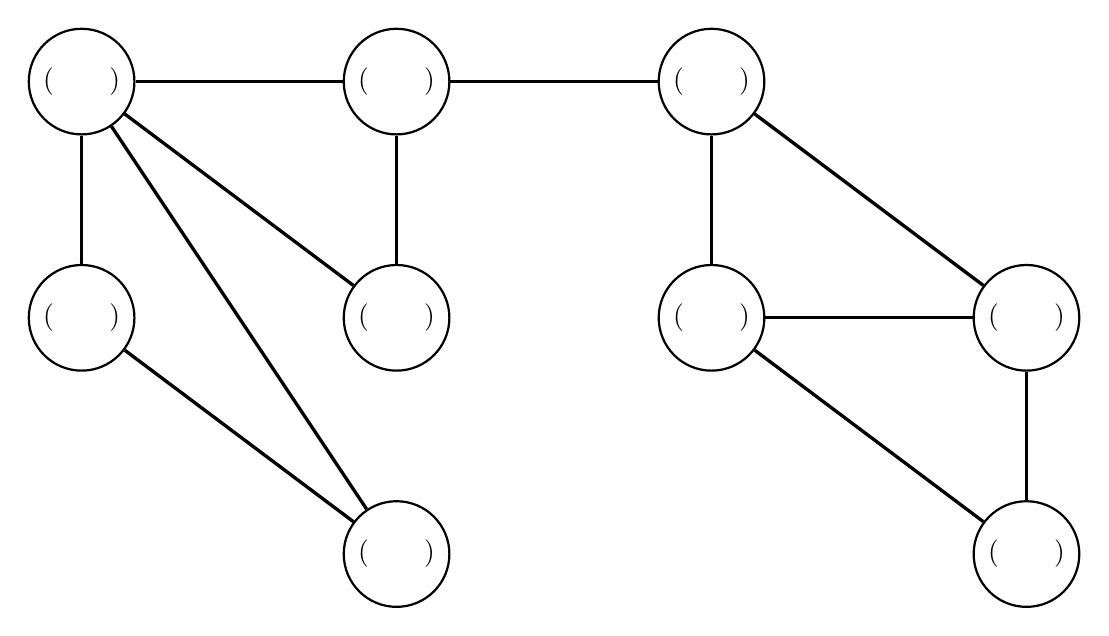
\begin{tikzpicture}
\begin{scope}[every node/.style={circle,thick,draw}]
    \node (v1) at (0,3) {(\qquad)};
    \node (v2) at (0,6) {(\qquad)};
    \node (v3) at (4,0) {(\qquad)};
    \node (v4) at (4,3) {(\qquad)};
    \node (v5) at (4,6) {(\qquad)};
    \node (v6) at (8,3) {(\qquad)};
    \node (v7) at (8,6) {(\qquad)};
    \node (v8) at (12,0) {(\qquad)};
    \node (v9) at (12,3) {(\qquad)};
\end{scope}
\begin{scope}[every node/.style={fill=white,circle},
              every edge/.style={draw=black,very thick}]
    \path (v1) edge (v2);
    \path (v1) edge (v3);
    \path (v2) edge (v3);
    \path (v2) edge (v4);
    \path (v2) edge (v5);
    \path (v4) edge (v5);
    \path (v5) edge (v7);
    \path (v6) edge (v7);
    \path (v6) edge (v8);
    \path (v6) edge (v9);
    \path (v7) edge (v9);
    \path (v8) edge (v9);
\end{scope}
\end{tikzpicture}

\newpage
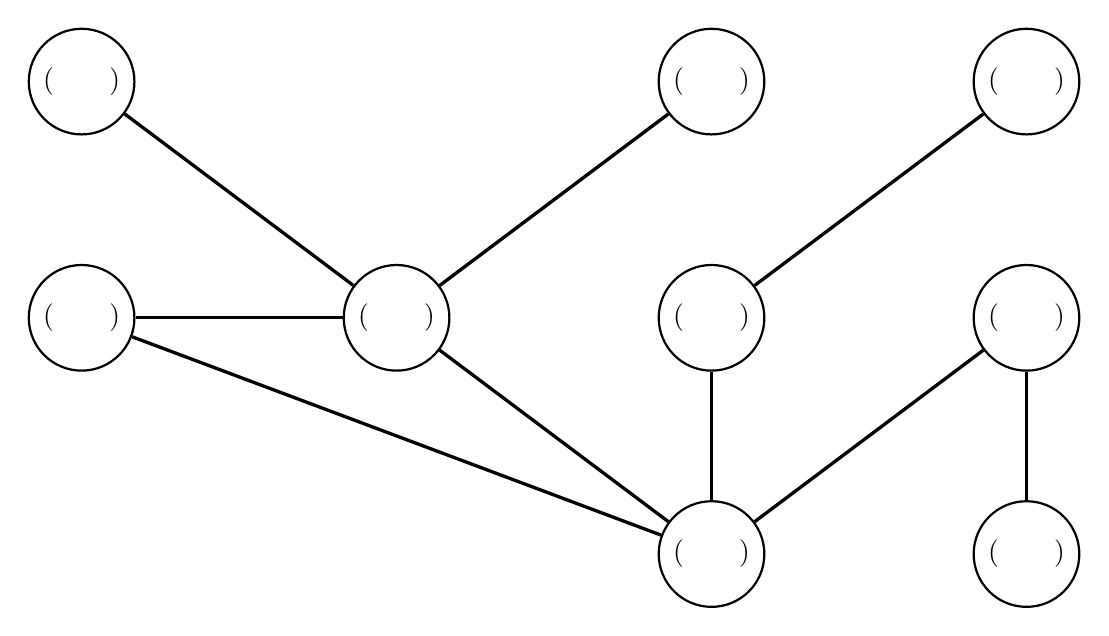
\begin{tikzpicture}
\begin{scope}[every node/.style={circle,thick,draw}]
    \node (v1) at (0,3) {(\qquad)};
    \node (v2) at (0,6) {(\qquad)};
    \node (v3) at (4,3) {(\qquad)};
    \node (v4) at (8,0) {(\qquad)};
    \node (v5) at (8,3) {(\qquad)};
    \node (v6) at (8,6) {(\qquad)};
    \node (v7) at (12,0) {(\qquad)};
    \node (v8) at (12,3) {(\qquad)};
    \node (v9) at (12,6) {(\qquad)};
\end{scope}
\begin{scope}[every node/.style={fill=white,circle},
              every edge/.style={draw=black,very thick}]
    \path (v1) edge (v3);
    \path (v1) edge (v4);
    \path (v2) edge (v3);
    \path (v3) edge (v4);
    \path (v3) edge (v6);
    \path (v4) edge (v5);
    \path (v5) edge (v9);
    \path (v7) edge (v8);
    \path (v8) edge (v4);
\end{scope}
\end{tikzpicture}

\vspace{2cm}
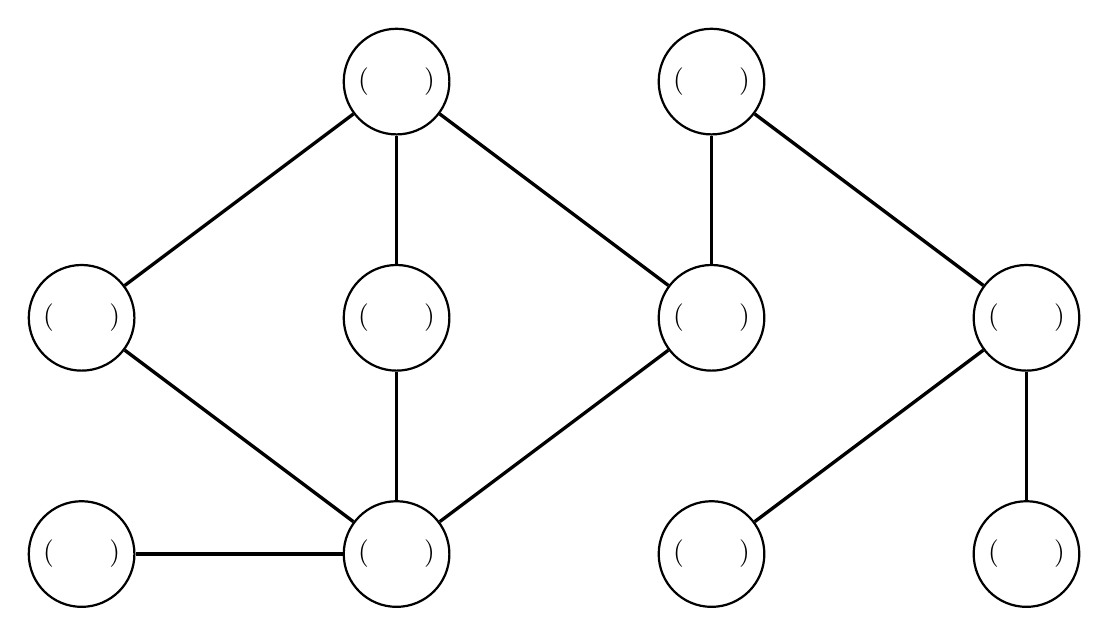
\begin{tikzpicture}
\begin{scope}[every node/.style={circle,thick,draw}]
    \node (v1) at (0,0) {(\qquad)};
    \node (v2) at (0,3) {(\qquad)};
    \node (v3) at (4,0) {(\qquad)};
    \node (v4) at (4,3) {(\qquad)};
    \node (v5) at (4,6) {(\qquad)};
    \node (v6) at (8,0) {(\qquad)};
    \node (v7) at (8,3) {(\qquad)};
    \node (v8) at (8,6) {(\qquad)};
    \node (v9) at (12,0) {(\qquad)};
    \node (v10) at (12,3) {(\qquad)};
\end{scope}
\begin{scope}[every node/.style={fill=white,circle},
              every edge/.style={draw=black,very thick}]
    \path (v1) edge (v3);
    \path (v2) edge (v3);
    \path (v2) edge (v5);
    \path (v3) edge (v4);
    \path (v3) edge (v7);
    \path (v4) edge (v5);
    \path (v5) edge (v7);
    \path (v6) edge (v10);
    \path (v8) edge (v7);
    \path (v8) edge (v10);
    \path (v9) edge (v10);
\end{scope}
\end{tikzpicture}

\newpage
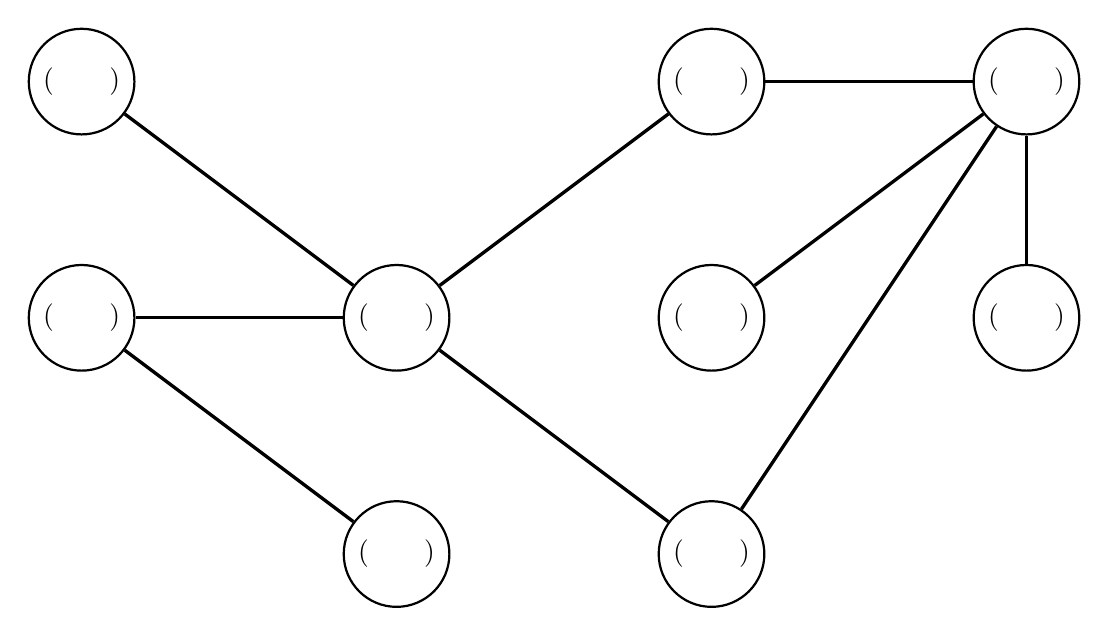
\begin{tikzpicture}
\begin{scope}[every node/.style={circle,thick,draw}]
    \node (v1) at (0,3) {(\qquad)};
    \node (v2) at (0,6) {(\qquad)};
    \node (v3) at (4,0) {(\qquad)};
    \node (v4) at (4,3) {(\qquad)};
    \node (v5) at (8,0) {(\qquad)};
    \node (v6) at (8,3) {(\qquad)};
    \node (v7) at (8,6) {(\qquad)};
    \node (v8) at (12,3) {(\qquad)};
    \node (v9) at (12,6) {(\qquad)};
\end{scope}
\begin{scope}[every node/.style={fill=white,circle},
              every edge/.style={draw=black,very thick}]
    \path (v1) edge (v4);
    \path (v1) edge (v3);
    \path (v2) edge (v4);
    \path (v4) edge (v5);
    \path (v4) edge (v7);
    \path (v5) edge (v9);
    \path (v6) edge (v9);
    \path (v7) edge (v9);
    \path (v8) edge (v9);
\end{scope}
\end{tikzpicture}

\vspace{2cm}
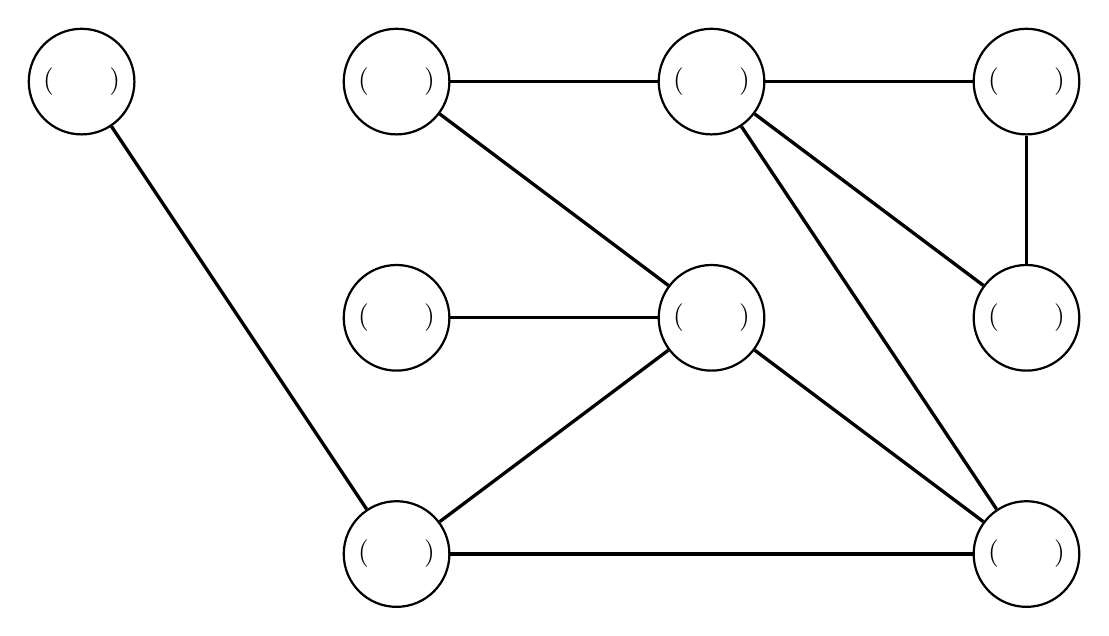
\begin{tikzpicture}
\begin{scope}[every node/.style={circle,thick,draw}]
    \node (v1) at (0,6) {(\qquad)};
    \node (v2) at (4,0) {(\qquad)};
    \node (v3) at (4,3) {(\qquad)};
    \node (v4) at (4,6) {(\qquad)};
    \node (v5) at (8,3) {(\qquad)};
    \node (v6) at (8,6) {(\qquad)};
    \node (v7) at (12,0) {(\qquad)};
    \node (v8) at (12,3) {(\qquad)};
    \node (v9) at (12,6) {(\qquad)};
\end{scope}
\begin{scope}[every node/.style={fill=white,circle},
              every edge/.style={draw=black,very thick}]
    \path (v1) edge (v2);
    \path (v2) edge (v5);
    \path (v2) edge (v7);
    \path (v3) edge (v5);
    \path (v4) edge (v5);
    \path (v4) edge (v6);
    \path (v5) edge (v7);
    \path (v6) edge (v8);
    \path (v6) edge (v9);
    \path (v6) edge (v7);
    \path (v8) edge (v9);
\end{scope}
\end{tikzpicture}

\end{document}